
\item A lamina is made by removing a small disc of diameter \( 2R \) from a bigger disc of uniform mass density and radius \( 2R \), as shown in the figure. The moment of inertia of this lamina about axes passing through \( O \) and \( P \) is \( I_{o} \) and \( I_{p} \), respectively. Both these axes are perpendicular to the plane of the lamina. The ratio \( \frac{I_{p}}{I_{o}} \) to the nearest integer is \underline{\hspace{2.5cm}}.

\begin{center}
    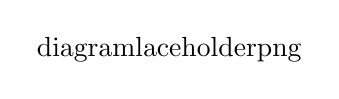
\begin{tikzpicture}
        % Diagram code will be here. For simplicity, we place a placeholder
        % as the specifics of the diagram are not provided.
        \node at (0,0) {diagramlaceholderpng};
    \end{tikzpicture}
\end{center}
